\documentclass[a4paper, 10pt, twocolumn, DIV=calc]{scrartcl}
\usepackage[T1]{fontenc}
\usepackage[utf8]{inputenc}
\usepackage{arsclassica}
\usepackage{graphicx}
\usepackage{booktabs}

\usepackage{geometry}
\geometry{top=1cm,bottom=1.5cm,left=2.5cm,right=2.5cm,includehead,includefoot}
\setlength{\columnsep}{7mm}


\usepackage{csquotes}
\usepackage[style=numeric,backend=biber]{biblatex}
\addbibresource{references.bib}

\begin{document}
\author{Group 4}
\title{Hate speech detection in Italian tweets}

\maketitle
\section{Introducion}
\subsection{Motivation}
Although hate speech is a phenomenon that existed long before the advent of the Web, communication via the Internet has allowed this phenomenon to spread and develop with peculiar characteristics tied to the nature of online media, such as anonymity on one side, and velocity and breadth of proliferation on the other. Given the relevance and dangerous potential of this social phenomenon, there is widespread interest in recognizing and detecting hate speech online, also on an institutional level.

In May 2016 the European Commission, citing the chilling effect of hate speech on the democratic discourse on online platforms,  agreed with Facebook, Microsoft, Twitter and YouTube on a ``Code of conduct on countering illegal hate speech online'' \cite{european_commission_code}.
In this document the major IT Companies made a public commitment to:
\begin{enumerate}
  \item Have in place clear and effective processes to review notifications regarding hate speech on their platforms;
  \item review the majority of valid notifications of hate speech in less than 24 hours.
\end{enumerate}

The most recent evaluation campaign of the Code of Conduct \cite{reynders_factsheet} assessed in general a worse performance of the IT Companies especially in this last respect (only 64.4\% of notifications were reviewed in less than 24 hours), confirming a troubling downward trend already observed in 2021.

Accurate, precise and efficient automated systems of hate speech detection are necessary for combating the phenomenon both with proactive action and in the process of reviewing user notification of occurrences of such violations.

Moreover, such systems should prove valuable for providing the data that is still needed to investigate the ecosystem of hate speech online and the magnitude of the phenomenon.
\subsection{Project goal}
The goal of this project is to identify characteristics in the text which allow for the detection of Italian tweets containing hate speech (this category is meant to include expressions of racism, xenophobia and terrorist propaganda).
So, we can define this task as a binary classification.

A secondary goal is to evaluate how insights obtained by our model can generalize across textual domains. In order to do that, we would like to test our model, trained exclusively on tweets, against Italian newspaper headlines.

The project is based on the main task of the HaSpeeDe 2 shared task presented at EVALITA2020 \cite{haspeede2}.

\section{Methods}
\subsection{Data}
We used the datasets made available\footnote{\url{https://github.com/msang/haspeede/tree/master/2020}} by the organizers of the Evalita 2020 shared task HaSpeeDe 2 \cite{haspeede2}.

The train set consists in 6839 Italian Tweets posted between October 2016 and May 2019 annotated for presence of hate speech.
The test set includes both a corpus of 1263 Italian Tweets posted between January and May 2019 and a corpus of 500 Italian newspapers' headlines retrieved between October 2017 and February 2018 from the online editions of \emph{La Stampa}, \emph{La Repubblica}, \emph{Il Giornale} and \emph{Liberoquotidiano}.
This second corpus will allow us to appraise how well the application generalizes across textual domains.

Table \ref{tbl:class_composition} shows the distribution of hate speech labels in the training set and in each of the test sets.

\begin{table}
\caption{Distribution of Hate Speech labels.}
    \begin{tabular}{lrrr}
        \toprule
        & \textsc{HS} & \textsc{Not HS} & \textsc{Total} \\
        \midrule
        Train & 2766 & 4073 & 6839 \\
        \midrule
        Test Tweets & 622 & 641 & 1263 \\
        Test News & 181 & 319 & 500 \\
        \bottomrule
    \end{tabular}
    \label{tbl:class_composition}
\end{table}

The data sets are available in TSV format and contain three features for each record:
\begin{itemize}
    \item{\texttt{id}:} numeric identifier for each document
    \item{\texttt{text}:} the body of the document
    \item{\texttt{hs}:} boolean value, whether the document contains HS (1) or not (0).
    \item{\texttt{stereotype}:} boolean value, whether the document contains a stereotype (1) or not (0) [might not be useful].
\end{itemize}

As part of the preprocessing performed by the organizers of the task, mentions and URLs recurring in the original documents were replaced with \texttt{@user} and \texttt{URL} placeholders.

We will also make use of the Italian Twitter embeddings \cite{italian_twitter_embeddings} lexicon computed by ItaliaNLP Lab on a corpus of 50,000,000 tweets using the word2vec\footnote{\url{http://code.google.com/p/word2vec/}} toolkit.
This lexicon consists of embeddings of 128 features for 1,188,949 tokens that were computed with the CBOW model with a symmetric context window of 5 tokens.

The embeddings were made available\footnote{\url{http://www.italianlp.it/download-italian-twitter-embeddings/}} by the ItaliaNLP Lab as a SQLite database containing a single table \texttt{store} with 130 columns:
\begin{itemize}
    \item \texttt{key}, representing the token;
    \item one column for each dimension of the embedding;
    \item \texttt{ranking} storing the frequency rank of the token.
\end{itemize}

\subsection{Automatic text annotation}
We automatically annotated the documents using a \emph{Stanza} \cite{stanza} pipeline: this operation consisted of:
\begin{itemize}
    \item Tokenization
    \item Part of speech tagging
    \item Lemma extraction
    \item Dependency parsing
\end{itemize}

Before this step we preprocessed the text in order to remove mentions, urls and normalize the punctuation: in particular sequences of multiple full stops were reduced to one full stop, since they were creating issues with the sentence tokenization.
As for hashtags, since often single words hashtags are integrated in the syntax of the sentence we decided to remove only the hash symbol and preserve the textual part of the hashtags.

Our choice of using Stanza was predicated on the possibility of using a combined model based on several different treebanks for the Italian language.
This allowed us to get a better coverage of the language, which is particularly important when working on a non standard variety like tweets or in general computer mediated writing.
In particular, the combined model is based on four treebanks ISDT, VIT, PoSTWITA and TWITTIRO: the latter two were developed specifically for the annotation of tweets.

\subsection{Linguistic profiling}
With the objective of identifying, if possible, stylistic features useful for hate speech detection, we developed 91 different features for the linguistic profiling of the text belonging to five different categories:

\begin{itemize}
    \item{\textbf{Raw text properties:}} text length in terms of number of tokens and number of sentences. Average length of sentences and words as a really simple proxy of syntactic complexity;
    \item{\textbf{Social media language properties:}} distribution of URLs, hashtags, mentions and all uppercase words;
    \item{\textbf{Lexical variety}} expressed in terms of Type/Token Ratio;
    \item{\textbf{Morpho-syntactic properties}}, namely the distribution of all grammatical categories and lexical density (proportion of content words in the text);
    \item{\textbf{Syntactic properties:}} distribution of all dependency relationships and relative order of core arguments and verb in sentences. Another aspect that received some attention was the distribution of nominal sentences, since the literature suggested a strong association between Slogan-like nominal utterances and hateful content \cite{comandini_nominal_utterances}.
\end{itemize}

In order to get some insights in the challenges associated with the cross-domain task, we scraped headlines from the online editions of \emph{La Stampa}, \emph{La Repubblica}, \emph{Il Giornale} and \emph{Liberoquotidiano}.
We filtered the headlines for the presence of the same small set of neutral keywords associated with immigrants, muslims and Roma used for the creation of the original dataset of tweets \cite{poletto_hate_2017}.

We thus obtained 748 newspapers headlines, which we passed to the automatic text annotation pipeline and analyzed stylistically.
We then trained a Linear Support Vector Machine on the linguistic profiling features in order to determine which features contributed the most in distinguishing between tweets and headlines. The classifier was able to distinguish tweets from headlines with near certainty, obtaining a macro-F1 of 0.949 in 5-fold cross validation.

As expected, social media properties like the number of mentions, hashtags, URLs and the use of uppercase, were mainly responsible for the success of the classifier. In addition to that, the feature importance analysis seems to indicate that tweets tend to be longer and have longer sentences than headlines; on the other hand, headlines seem to use more punctuation and more proper nouns and exhibit higher lexical variety (but since the Type/Token Ratio measure is highly sensitive to text length, this is probably a spurious result).
Figure \ref{fig:style} shows the distributions of several linguistic profiling features (document length in tokens, average sentence length, distribution of punctuation, distribution of proper nouns and Type/Token Ratio by form) for tweets and headlines.
Although the distributions are overlapping, it is possible to discern clear trends that confirm the results of the feature importance analysis.

\begin{figure}
    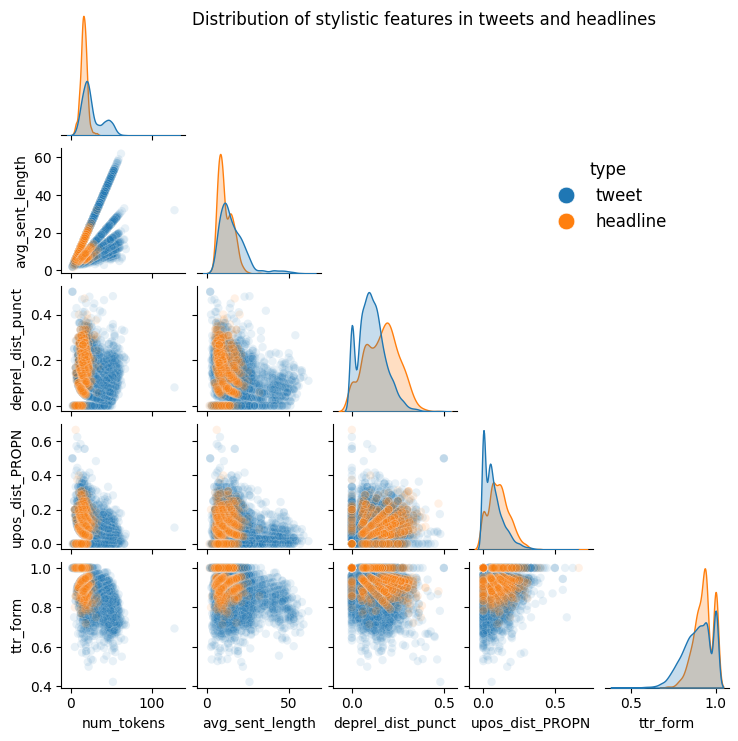
\includegraphics[width=\columnwidth]{../../results/images/style.png}
    \caption{Comparat{}ive stylistic analysis of tweets and scraped headlines.}
    \label{fig:style}
\end{figure}
\subsection{Ngrams extraction and modelling}

In this section, we describe the process used to extract n-grams from tweets to exploit them as features.
The process begins with a pre-processing step applied to the raw training dataset, implemented through the \texttt{clean\_df function}, which consists of three inner functions.The first inner function, \texttt{count\_uppercase}, calculates the number of uppercase characters in the dataset.
When we considered the stylistic features, we successfully replaced this simple counter with a function that computes the ratio between uppercase and lowercase characters.

Additionally, we defined a custom punctuation set that extends the standard \texttt{string.punctuation} by including special characters encountered in tweets. After applying this function, the dataset includes the original columns, text and hs, along with a new column,\texttt{ uppercase\_count}.

The second inner function, \texttt{split\_hashtags}, utilizes the \emph{WordSegment} library to split words within hashtags. This function is stochastic, meaning it may split hashtags differently during each execution. Based on our observations, the function performs well in identifying and splitting longer words within hashtags but struggles with stopwords and shorter words.
This second inner function is incorporated into the \texttt{process\_hashtags} function, which tokenizes hashtags when more than one word is present.
An additional condition was added to handle words longer than 10 characters, although this could occasionally split valid long words incorrectly.
However, given the rarity of such words in the dataset, this approach is effective for identifying incorrectly joined words.
At this stage, the dataset includes a new column, \texttt{text\_processed}.

Subsequently, all text is converted to lowercase, mentions, URLs, and numbers are removed, and the tweets are tokenized using \emph{Stanza} \cite{stanza}.
Tokens are then further processed by removing stopwords and punctuation.
After tokenization, two additional columns are added: one reporting the final number of tokens per tweet and another counting the occurrence of bad words, if any, from the list of 500 Italian badwords.

Once the tokenized version of the tweets was prepared, we lemmatized the tokens to ensure higher consistency and reduce the number of final n-grams.
Given the brevity of tweets, we limited the n-grams to unigrams and bigrams.

The final dataset consisted of 6837 rows and 6407 features, including the original tweet, tokenized version, lemmatized version, the number of uppercase characters, the count of bad words, and extracted unigrams and bigrams. Before extracting additional features and embeddings, we conducted initial experiments by training models directly on this dataset.
Several models were tested, including Random Forest, SVM, XGBoost, and Logistic Regression using as features only n-grams and badword counts. After applying random search for hyperparameter tuning, the best performance was achieved with Logistic Regression, yielding a macro average F1 score of 0.743.
In this step we didn’t use the Select KBest for selecting the best k features because otherwise the model couldn’t be used properly on the test, so we used all the features.

The same preprocessing steps used for the training set were applied to both test sets: one containing tweets and the other containing 500 headlines from Italian newspapers. To ensure consistency between the test datasets and the training set, we used the dictionary, the Bigram model, and the TF-IDF model fitted on the training set.
As a result, the final test datasets have the same number of features as the training set. This ensures that the model trained on the training dataset can be correctly applied to the test set. Specifically, if an n-gram is present in both the training and test sets, the corresponding column will report non-zero values; otherwise, the column will consist entirely of zeros. Additionally, by using the same TF-IDF model for both training and testing, the weight of each n-gram remains consistent.

SPOSTA IN RESULTS

\subsection{Embeddings}
\label{subsec:Embeddings}
Among the approaches we decided to implement, we opted for an SVM classifier trained using embeddings-based textual representations. 

We first tested three different representations based on the same lexicon of  precomputed static word embeddings, the Italian Twitter Embeddings \cite{italian_twitter_embeddings} by the ItaliaNLP Lab, differing by method of aggregation. 

In order to do so, we loaded the embeddings and our preprocessed and annotated training documents, which we further normalized using the functions provided by the ItaliaNLP lab. We could then build the vocabulary of the training set using the embeddings. Given the characteristics of this type of non-standard language, in particular the high level of both inter and intrapersonal variation, we expected some out-of-vocabulary words, which ended up being 2703 out of 22709, meaning that almost 12\% of words didn't have an embedding representation. These words are mostly words that haven't been correctly tokenized (especially multi-words hashtags), sequences of emojis, and typos. Had we used non-specialized embeddings, we assume that this coverage would have been significantly lower, posing an important issue for the model training.

Using a 5-fold cross-validation process and comparing the resulting macro-averaged F1 score, we determined the best performing model to be the one representing each tweet with the average of all its word embeddings. It performed better than using the aggregation of only lexically-full tokens (nouns, verbs and adjectives), both by mean and by concatenation of the mean vectors for the three aforementioned grammatical categories.

\begin{table}
    \begin{tabular}{rlr}
        \toprule
        & \textsc{Features} & \textsc{Macro F1} \\
        \midrule
        1 & Avg over all tokens & 0.744 \\
        2 & Avg over all N, V and Adj & 0.726 \\
        3 & Concat. of mean vects (N, V, Adj) & 0.717 \\
        \bottomrule
    \end{tabular}
    \caption{SVM classifiers based on different word embeddings aggregations (5-fold cross-validation).}
    \label{tbl:svm_f1_static_embs_aggregations}
\end{table}

We then followed the same methodology to test representations based on contextual embeddings extracted from two different Italian pre-trained BERT models. \footnote{\textbf{BERT} (Bidirectional Encoder Representations from Transformers) is a bidirectional Large Language Model (LLM) based on an encoder-only transformer architecture. This Deep Learning model was presented by Google in 2018.}
\begin{enumerate}
    \item \textbf{dbmdz/bert-base-italian-cased} or (\textbf{Italian BERT}) \cite{italian_bert}:  trained on a corpus consisting of a Wikipedia dump and texts from the OPUS corpora collection, for a total of 2,050,057,573 tokens.
    \item \texttt{\textbf{m\_polignano\_uniba/bert\_uncased\_L{-}12\_H{-}\allowbreak768\_A{-}12\_italian\_alb3rt0}} (or \textbf{AlBERTo}) \cite{alberto}:  the first Italian BERT model for Twitter language understanding, trained on Italian tweets.
\end{enumerate}

For both models, we tested two methods of \textit{pooling} the tokens' embedding representations generated by the model after processing the input sequence into a single sentence embedding for each tweet (or, more generally, document).
\begin{enumerate}
    \item \textbf{[CLS] pooling}: the model's tokenizer adds the special token [CLS] at the start of every sequence. During the training process of the Large Language Model, its embedding (or hidden state) will capture sequence-level information. By extracting the [CLS] token's embedding of each document from the final hidden layer, we obtain a representation that can serve as a sentence-level embedding.
    \item \textbf{Mean Pooling with Sentence Transformers}: we used a Sentence Transformer, a model that generates a single fixed-length vector representation for an entire sequence. It does so via \textit{mean pooling}, i.e. by computing the mean of all tokens' embeddings in the last hidden layer.
\end{enumerate}

The Italian BERT yielded worse performances, which can be explained by the fact that it is a general model that has not been trained for this specific domain. AlBERTo, on the other hand, provided better results, with the SVM model based on its mean pooled embeddings having the highest mean macro F1 score.
    
\begin{table}
\centering
    \begin{tabular}{lrr}
        \toprule
        & \textsc{[CLS]} & \textsc{Mean Pooling} \\
        \midrule
        Italian BERT & 0.689 & 0.725 \\
        AlBERTo & 0.741 & 0.747 \\
        \bottomrule
    \end{tabular}
    \caption{Mean macro F1 score of SVM classifiers based on different contextual embeddings' poolings (5-fold cross-validation).}
    \label{tbl:svm_f1_contextual_embs_pooling}
\end{table}

\subsection{Handling Emoji}

\subsubsection{Introduction}
Analyzing emoji in Italian tweets is essential for understanding expressiveness, sentiments, and the main topics shared online. Emoji represent a unique form of communication that complements textual language with visual symbols to convey emotions, emphasis, and cultural context. Our objectives are therefore to:
\begin{itemize}
    \item Identify emoji usage patterns in Italian tweets.
    \item Analyze the frequency and distribution of emoji.
    \item Explore the semantic meaning of emoji in relation to textual content.
    \item Apply clustering techniques to categorize tweets based on emoji usage.
\end{itemize}

\subsubsection{Dataset and Preprocessing}
To ensure the quality of the analysis, the dataset was pre-processed:
\begin{enumerate}
    \item \textbf{Removal of superfluous elements}: Mentions (\texttt{@user}), URLs, hashtags, and non-decodable characters were removed.
    \item \textbf{Text normalization}: All text was converted to lowercase, and redundant spaces were removed.
    \item \textbf{Tokenization}: The text was separated into individual words or symbols for detailed analysis.
    \item \textbf{Emoji extraction}: The \texttt{emoji} library was used to identify and isolate emoji symbols from the text.
\end{enumerate}

\subsubsection{Extraction and Analysis}
We performed two different extractions—one for emoticons and one for emoji. For the former, it was necessary to set a pattern to identify them; for the latter, it was carried out via tokenization and recognition patterns provided by the \texttt{emoji} library. The following analyses were conducted:
\begin{itemize}
    \item \textbf{Emoji counting}: Calculation of the frequency of each emoji in the dataset.
    \item \textbf{Meaning mapping}: Linking emoji to their descriptive names and semantic meanings.
    \item \textbf{Emoji distribution}: Statistical analysis to identify the most common emoji.
    \item \textbf{Relationship with textual content}: Exploration of the correlation between emoji usage and the topics discussed in tweets.
\end{itemize}

\subsubsection{Visualization and Results}
The main visualizations developed include:
\begin{enumerate}
    \item \textbf{Emoji frequency}: A bar chart showing the most used emoji in the dataset.
    \item \textbf{Clustering}: Use of algorithms such as \texttt{K-Means} and \texttt{PCA} to identify groups of tweets based on common emoji usage patterns.
\end{enumerate}
\begin{figure}
    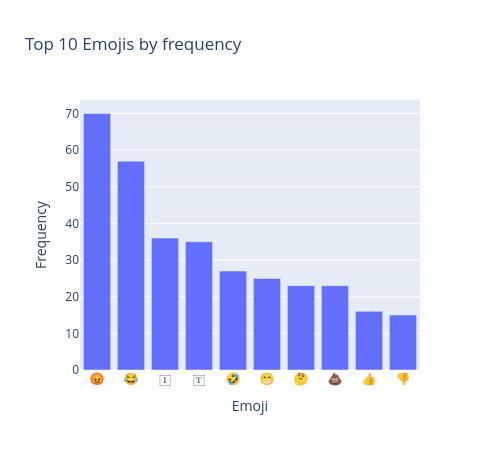
\includegraphics[width=\columnwidth]{../../results/images/emoji_top10.png}
    \caption{Distribution of the most frequent emoji in tweets.}
    \label{fig:emoji_frequenze}
\end{figure}
As we can see from the bar chart, the most frequently used emoji is the enraged face. This chart is very helpful in understanding the trend among the tweets under analysis. As expected, the most prominent sentiment is anger. Subsequent results are also significant, showing the laughing face and then the “IT” pair of emoji. When combined, these emoji might suggest the prevalence of sarcasm, anger, and blame directed toward the state.

\subsubsection{TF-IDF for Emoji and Emoticon Analysis}
One of the key techniques applied was the use of TF-IDF (Term Frequency–Inverse Document Frequency) to analyze the meaning and importance of both emoji and emoticons in relation to the textual content of the tweets. The process was structured as follows:
\begin{enumerate}
    \item \textbf{Text tokenization}: Each tweet was divided into tokens, including both emoji and emoticons.
    \item \textbf{Generation of n-grams}: For each emoji-emoticon, n-grams (from 1-gram to 5-gram) were generated to analyze combined usage patterns.
    \item \textbf{Frequency calculation}: The relative frequency (TF) of each n-gram was calculated within each tweet.
    \item \textbf{Inverse weighting calculation}: The relative importance of each n-gram in the corpus was calculated, penalizing those present in all tweets (IDF).
    \item \textbf{Vectorization}: Each tweet was represented as a TF-IDF vector, where each dimension corresponds to an n-gram.
    \item \textbf{Parameter optimization}: The optimal value of \textit{n} (the length of the n-grams) was chosen based on total frequency.
\end{enumerate}
Implementing TF-IDF made it possible to distinguish generic symbols with common meanings from those that are more specific and characterize particular themes or emotions.

\subsubsection{Results of the TF-IDF Analysis}
Applying TF-IDF highlighted the following main n-grams with their corresponding TF-IDF values:

\begin{table}[!h]
    \centering
    \begin{tabular}{lc}
    \toprule
    \textbf{N-gram} & \textbf{TF-IDF} \\
    \midrule
    enraged\_face & 0.003181 \\
    italy & 0.002182 \\
    face\_with\_tears\_of\_joy & 0.002172 \\
    thinking\_face & 0.001885 \\
    xo & 0.001316 \\
    pile\_of\_poo & 0.001268 \\
    rolling\_on\_the\_floor\_laughing & 0.001136 \\
    beaming\_face\_with\_smiling\_eyes & 0.001036 \\
    d & 0.001024 \\
    enraged\_face\_enraged\_face & 0.000979 \\
    \bottomrule
    \end{tabular}
    \caption{Top n-grams of emoji names with corresponding TF-IDF values.}
    \label{tab:tfidf_results}
\end{table}

\subsubsection{Comparison of Emoji in Tweets With and Without Hate Speech}
A comparison of the emoji used in tweets with and without hate speech was carried out to analyze differences and specific patterns. The relative frequencies of emoji were calculated in both datasets:
\begin{itemize}
    \item \textbf{Tweets with Hate Speech (HS)}: Includes tweets where \texttt{hs} $= 1$.
    \item \textbf{Tweets without Hate Speech (NHS)}: Includes tweets where \texttt{hs} $= 0$.
\end{itemize}
Emoji frequencies were represented graphically for each group:

\begin{figure}
    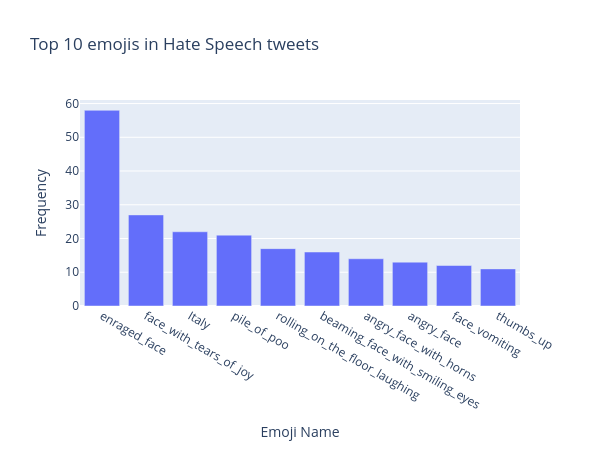
\includegraphics[width=\columnwidth]{../../results/images/emoji_top10_hs.png}
    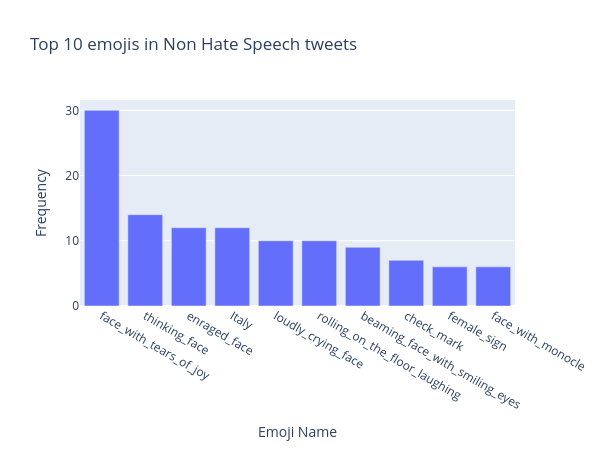
\includegraphics[width=\columnwidth]{../../results/images/emoji_top10_nhs.png}
    \caption{Top 10 Emoji in Tweets With and Without Hate Speech.}
    \label{fig:hs_emoji}
\end{figure}
As we can see in Figure \ref{fig:hs_emoji}, emoji such as “Italy,” “face\_with\_tears\_of\_joy,” “enraged\_face,” etc., appear in both rankings and also at the top positions. This suggests that the enraged face emoji can sometimes be used to express emotions of disappointment, political fatigue, and distrust regarding the topic of immigration. Conversely, the presence of the laughing emoji in the first ranking is indicative of malevolent sarcasm, mockery, and frustration. A similar observation applies to the Italian flag emoji, which is often used in both types of tweets.
\newpage
\subsubsection{Tweet Clustering}
Clustering was performed to categorize tweets based on emoji and emoticons. The main steps were:
\begin{enumerate}
    \item \textbf{Data transformation}: We used the TF-IDF vectors based on the emoji names created before.
    \item \textbf{Determining the optimal number of clusters}: The \textit{Elbow} method was used to find the optimal value of \( k \). Figure~\ref{fig:elbow_method} shows the Elbow method plot.
    \item \textbf{Dimensionality reduction}: \texttt{Principal Component Analysis} (PCA) was applied to reduce the data to three dimensions for visualization.
    \item \textbf{Clustering}: The \texttt{K-Means} algorithm was used to identify four distinct clusters based on emoji usage.
\end{enumerate}

\begin{figure}
    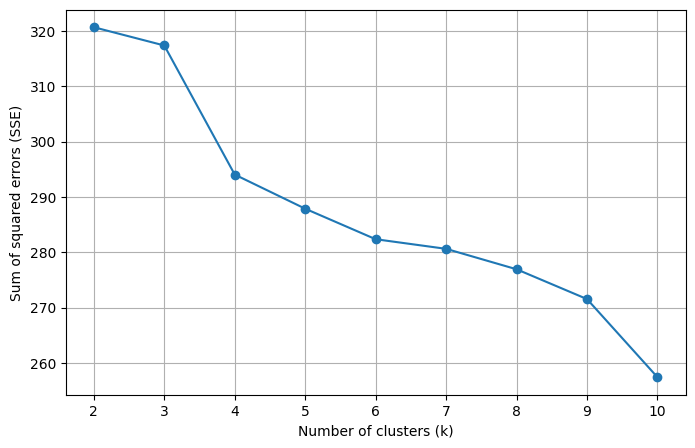
\includegraphics[width=\columnwidth]{../../results/images/emoji_elbow.png}
    \caption{Elbow Method for Determining the Optimal Number of Clusters.}
    \label{fig:elbow_method}
\end{figure}

\begin{figure}
    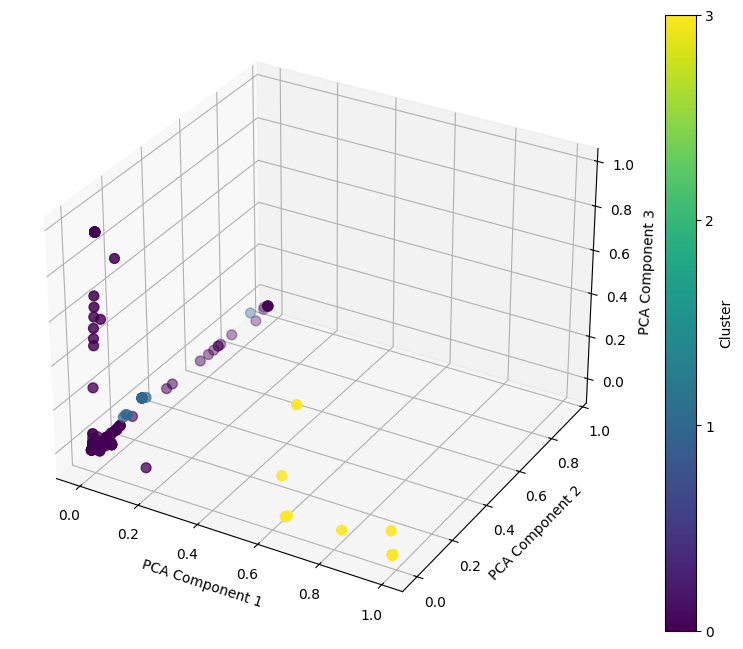
\includegraphics[width=\columnwidth]{../../results/images/emoji_cluster.png}
    \caption{K-Means Emoji Clustering (k=4) – 3D Visualization.}
    \label{fig:3d_clustering}
\end{figure}

Figure~\ref{fig:3d_clustering} shows the cluster distribution in a three-dimensional space based on the computed principal components.

The results show that emoji are not easily clusterable. Even though the optimal \( k \) found is 4, we end up with only 3 actual clusters. This is due to the nature of the available data. The division seems to be on the vertical layer and, based on the trend of the obtained data, we can hypothesize that the blue cluster contains emojis with negative sentiment, the yellow cluster contains those with positive sentiment, and the magenta cluster comprises neutral emoji used in tweets featuring hate speech. These are hypotheses since we are not able to derive more relevant information.

\subsection{Models}

The train set used for this phase of exploring various classifiers consists mainly of four datasets: unigrams and bigrams, embeddings, stylistic features, and the offensiveness score. Depending on which embeddings dataset is used the dimensionality may change, but in general it is around 7000 total features.
{}
After tuning the hyperparameters of several classifiers (Logistic Regression, SVM, Random Forest, XGBoost, Light-GBM) the best one turned out to be Light-GBM (with an average F1-macro of 0.774 on 5 folds of cross-validation), as well as being clearly the fastest. Thus, we used this first version of the model to carry out several analyses regarding features.
For example, with respect to feature importance: although any of the four datasets manages, taken individually for training, to achieve an average F1-macro of at least 0.75, when used all together the model takes into account almost only the embeddings to classify (and a few other interesting features such as the unigrams 'rom' and 'terrorism', the stylistic features 'uppercase\_words\_dist' and 'lexical\_density', and 'offensiveness\_score' and 'badword').
Moreover, thanks to the calculation of feature importance, we were able to observe that the model does not benefit at all from many of our features, as it achieves its highest result (average F1-macro of 0.784) using only the first 100, as shown by the plot at figure \ref{fig:features}.

\begin{figure}
    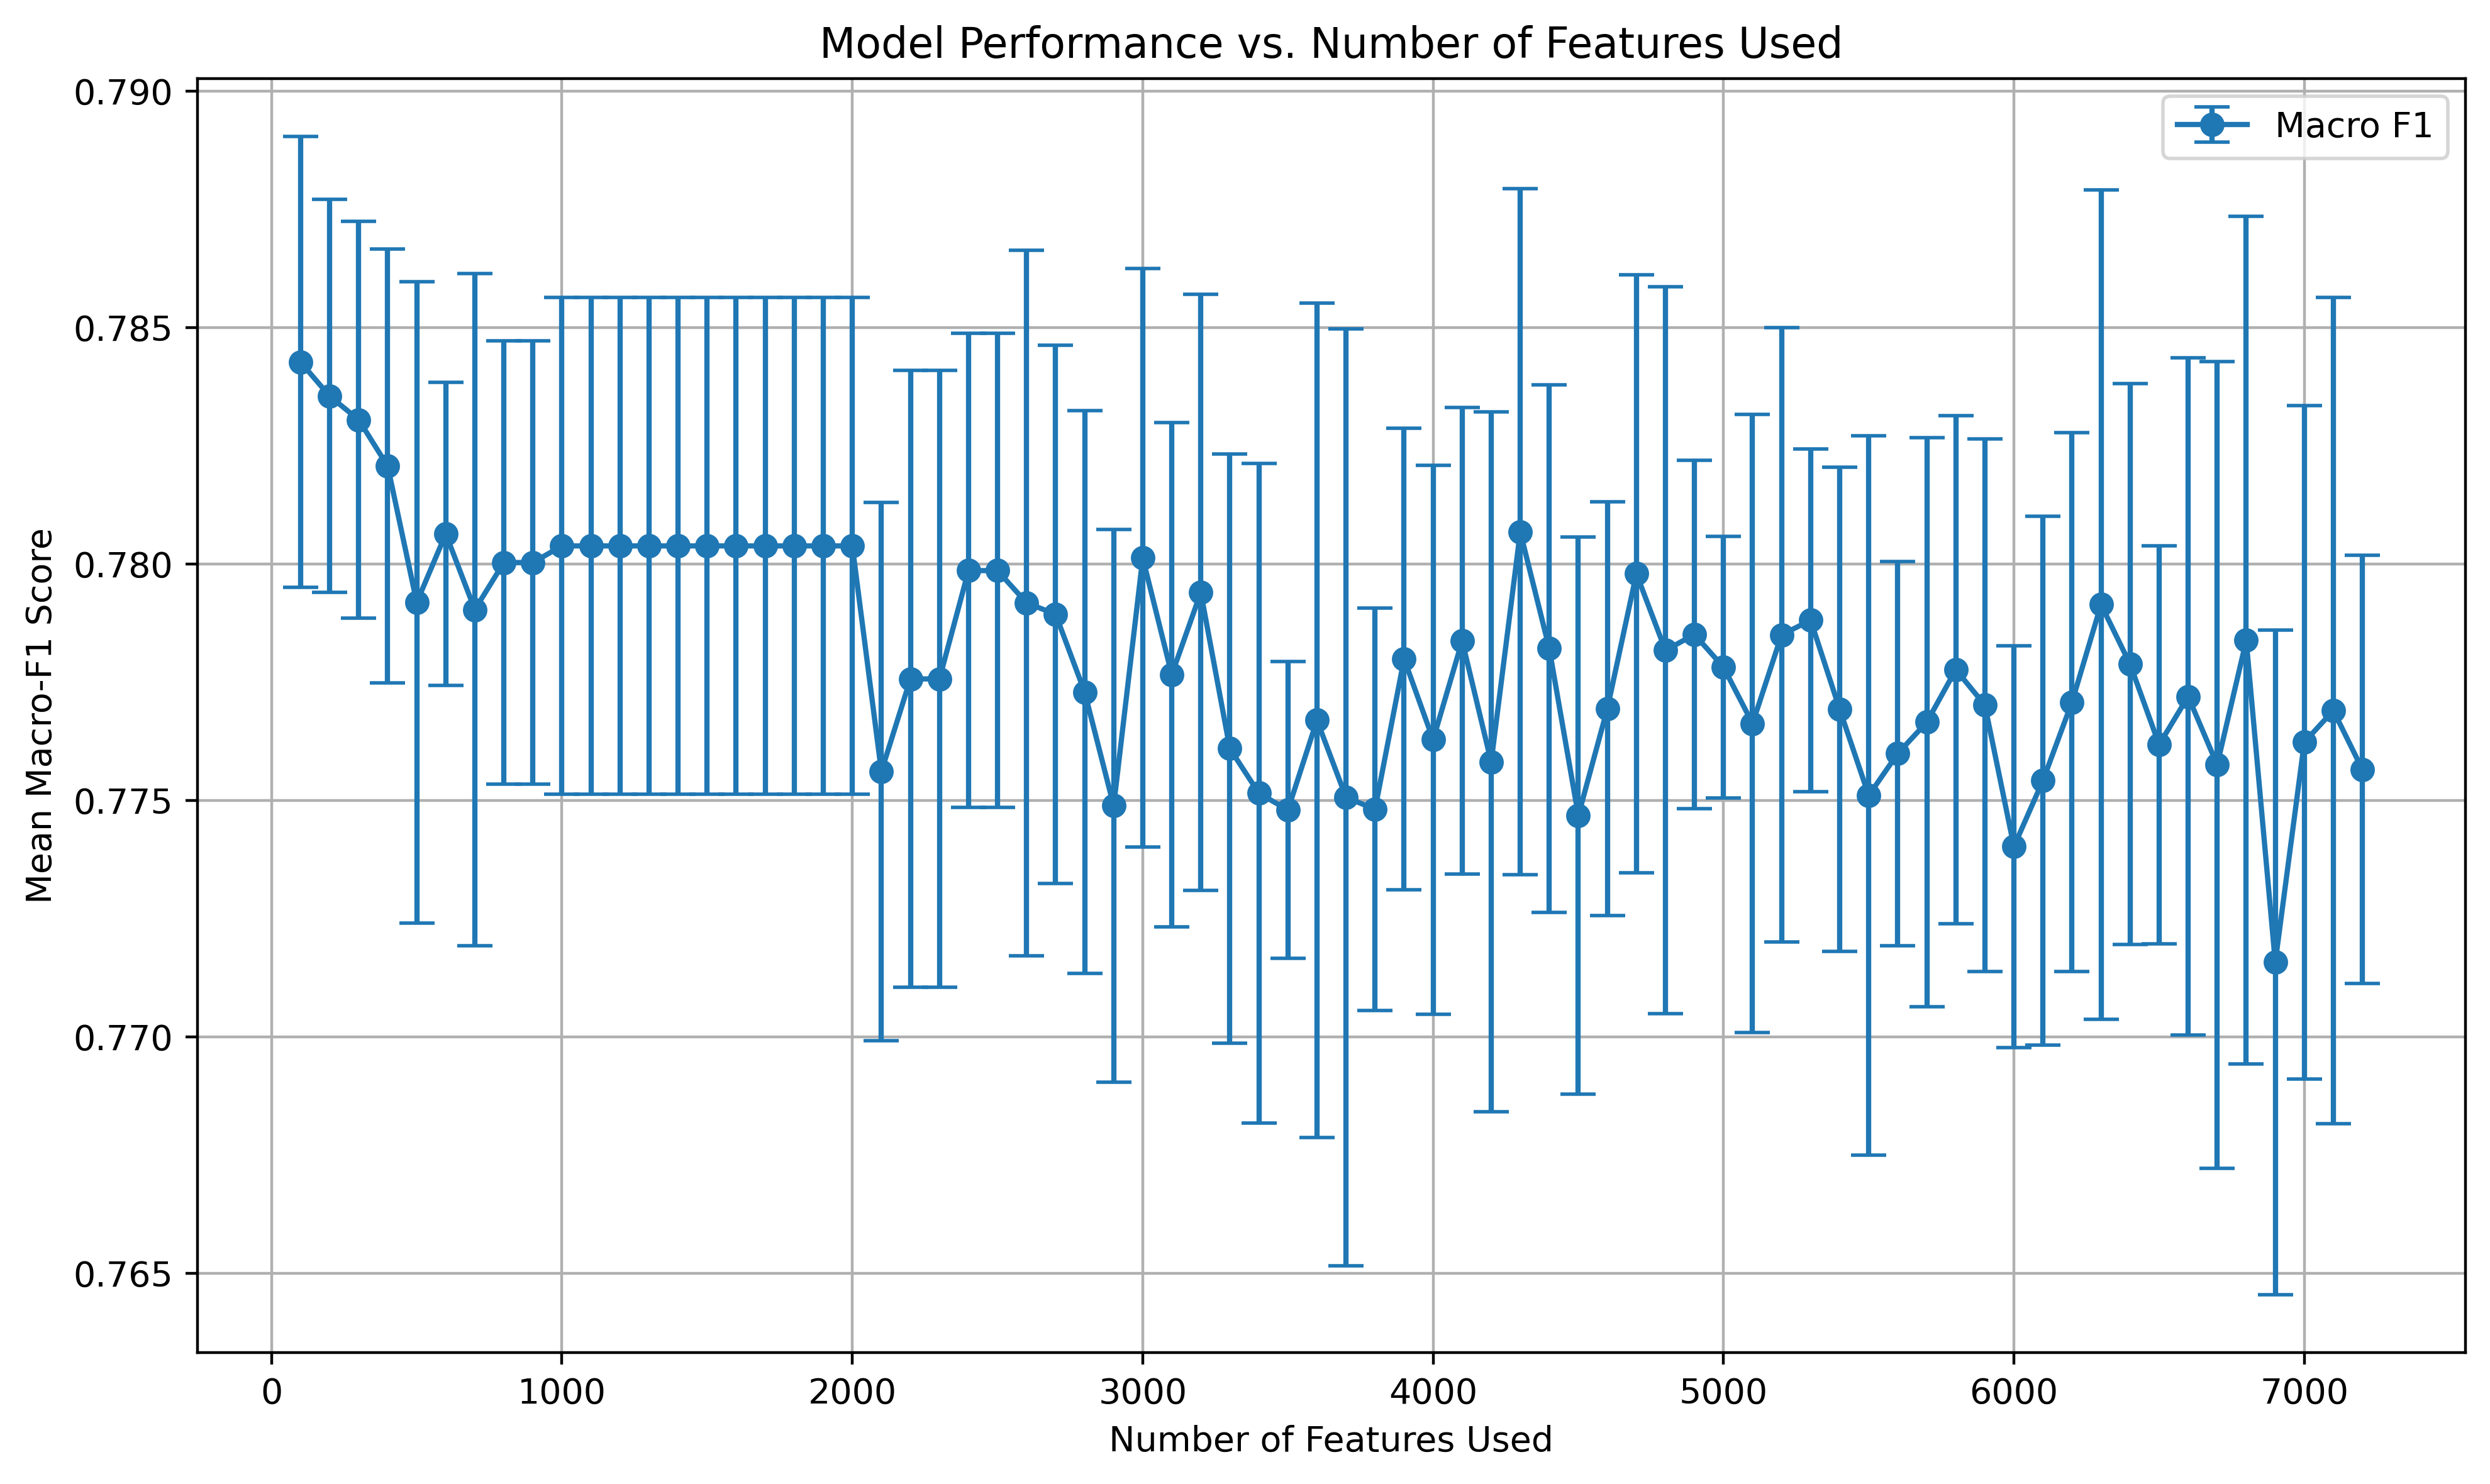
\includegraphics[width=\columnwidth]{../../results/images/model_n_feats.png}
    \caption{Performance of LGBM classifier vs number of features used by the classifier}
    \label{fig:features}
\end{figure}
Regarding embeddings, since they are apparently the most useful feature set, we trained the model on all the embeddings datasets we computed to check if there is any noticeable difference, and we found that the one that best performing embeddings are the mean pooled embeddings from AlBERTo.

With regard to the offensiveness score, we found instead that the score normalized by the length of the tweet returned better results than the non-normalized score and than both scores used together.

Finally, after all the information obtained, we performed a more comprehensive randomized search to re-tune the hyperparameters of the Light-GBM in order to have a definitive model to use for testing (the model reached an average F1-macro of 0.778 on the validation set). For the generalisation task, since the stylistic features are very different between tweets and newspaper headlines, we decided to perform a second tuning to generate another model that is not trained on stylistic features.

\section{Results}
\section{Discussion}
\section{Conclusion}

\printbibliography{}

\end{document}